%
% Documento: Apêndices
%

\begin{apendicesenv}

\chapter{ESPECIFICAÇÕES DOS CASOS DE USO}\label{especCdU}

\begin{table}[!h]
	\begin{center}
		\caption{Especificação do caso de uso Gerenciar Animais}
		\begin{tabular}{ | l |  p{10cm} |}
			\hline
			Código e Nome do Caso de Uso & CdU001 - Gerenciar Animais \\ \hline
			Ator Primário: & Usuário \\
			Ator Secundário: & Não se aplica \\ \hline
			Fluxo Principal de Eventos & P1. O usuário solicita consultar os animais. \\
						   & P2. O sistema apresenta a tela de animais. (IV003) (A1) (A2) \\
						   & P3. O usuário solicita ver um animal em específico. \\
						   & P4. O sistema apresenta a tela de perfil do animal. (IV006) (A3) (A4)  \\
						   & P5. O caso de uso se encerra. \\ \hline
			Fluxo Alternativo:         & A1.1. Em P2 o usuário insere as informações de um animal no formulário e solicita salvá-las. \\
			A1. Adicionar animal       & A1.2. O sistema salva o animal. \\
						   & A1.3. Retorna ao P2. \\ \hline
			Fluxo Alternativo:         & A2.1. Em P2 o usuário tem a intenção de deletar um animal. \\
			A2. Deletar animal         & A2.2. O sistema apaga o animal selecionado. \\
						   & A2.3. Retorna ao P2. \\ \hline
			Fluxo Alternativo:         & A3.1. Em P4 o usuário decide editar animal. \\
			A3. Editar animal          & A3.2. O sistema apresenta a tela de editar animal. (IV007) \\
						   & A3.3. O usuário insere as novas informações do animal. \\
						   & A3.4. O sistema salva essas informações. \\
						   & A3.5. Retorna ao P4. \\ \hline
			Fluxo Alternativo:         & A4.1. Em P4 o decide adicionar uma nova pesagem do animal. \\
			A4. Adicionar peso         & A4.2. O sistema apresenta a tela de adicionar pesagem. (IV008) \\
						   & A4.3. O usuário insere as novas informações de peso do animal. \\
						   & A4.4. O sistema salva essas informações. \\
						   & A4.3. Retorna ao P4. \\ \hline
			Fluxo Alternativo:         & A5.1. Em P4 o usuário decide consultar detalhes do animal. \\
			A5. Consultar Detalhes     & A5.2. O sistema apresenta a tela de detalhes do animal. \\
						   & A5.3. Retorna ao P4. \\
			\hline
		\end{tabular}
		Fonte: Autoria própria.
	\end{center}
\end{table}

\newpage

\begin{table}[!h]
	\begin{center}
		\caption{Especificação do caso de uso Gerenciar Remédios}
		\begin{tabular}{ | l |  p{10cm} |}
			\hline
			Código e Nome do Caso de Uso & CdU002 - Gerenciar Remédios \\ \hline
			Ator Primário: & Usuário \\
			Ator Secundário: & Não se aplica \\ \hline
			Fluxo Principal de Eventos & P1. O usuário solicita consultar os remédios. \\
						   & P2. O sistema apresenta a tela de remédios. (IV004) (A1) (A2) (A3) \\
						   & P3. O caso de uso se encerra. \\ \hline
			Fluxo Alternativo:         & A1.1. Em P2 o usuário insere as informações de um remédio no formulário e solicita salvá-las. \\
			A1. Adicionar remédio      & A1.2. O sistema salva o remédio. \\
						   & A1.3. Retorna ao P2. \\ \hline
			Fluxo Alternativo:         & A2.1. Em P2 o usuário resolve deletar um remédio. \\
			A2. Deletar remédio        & A2.2. O sistema apaga o remédio selecionado. \\
						   & A2.3. Retorna ao P2. \\ \hline
			Fluxo Alternativo:         & A3.1. Em P2 o usuário decide editar um remédio. \\
			A3. Editar remédio         & A3.2. O sistema apresenta a tela de editar remédio. \\
						   & A3.3. O usuário insere as novas informações do remédio. \\
						   & A3.4. O sistema salva essas informações. \\
						   & A3.5. Retorna ao P2. \\
			\hline
		\end{tabular}
		Fonte: Autoria própria.
	\end{center}
\end{table}

\begin{table}[!h]
	\begin{center}
		\caption{Especificação do caso de uso Visualizar Relatórios}
		\begin{tabular}{ | l |  p{10cm} |}
			\hline
			Código e Nome do Caso de Uso & CdU003 - Visualizar Relatórios \\ \hline
			Ator Primário: & Usuário \\
			Ator Secundário: & Não se aplica \\ \hline
			Fluxo Principal de Eventos & P1. O usuário solicita consultar os relatórios. \\
						   & P2. O sistema apresenta a tela de relatórios da fazenda. \\
						   & P3. O caso de uso se encerra. \\
			\hline
		\end{tabular}
		Fonte: Autoria própria.
	\end{center}
\end{table}

\newpage

\begin{table}[!h]
	\begin{center}
		\caption{Especificação do caso de uso Gerenciar Medicação}
		\begin{tabular}{ | l |  p{10cm} |}
			\hline
			Código e Nome do Caso de Uso & CdU004 - Gerenciar Medicação \\ \hline
			Ator Primário: & Usuário \\
			Ator Secundário: & Não se aplica \\ \hline
			Fluxo Principal de Eventos & P1. O usuário solicita consultar medicação. \\
						   & P2. O sistema apresenta a tela de medicação. (IV005) (A1) (A2) (A3) \\
						   & P3. O caso de uso se encerra. \\ \hline
			Fluxo Alternativo:         & A1.1. Em P2 o usuário insere as informações de uma medicação e solicita salvá-las. \\
			A1. Adicionar medicação    & A1.2. O sistema salva a medicação. \\
						   & A1.3. Retorna ao P2. \\ \hline
			Fluxo Alternativo:         & A1.1. Em P2 o usuário resolve deletar uma medicação. \\
			A2. Deletar medicação      & A2.2. O sistema apaga a medicação selecionada. \\
						   & A2.3. Retorna ao P2. \\ \hline
			Fluxo Alternativo:         & A3.1. Em P2 o usuário decide editar uma medicação. \\
			A3. Editar medicação       & A3.2. O sistema apresenta a tela de editar medicação. \\
						   & A3.3. O usuário insere as novas informações da medicação. \\
						   & A3.4. O sistema salva essas informações. \\
						   & A3.5. Retorna ao P2. \\
			\hline
		\end{tabular}
		Fonte: Autoria própria.
	\end{center}
\end{table}


\chapter{DIAGRAMAS DE ATIVIDADE}\label{ativ}
\begin{figure}[H]
	\begin{center}
		\caption{Diagrama da Atividade de Gerenciar Animal parte 1}
		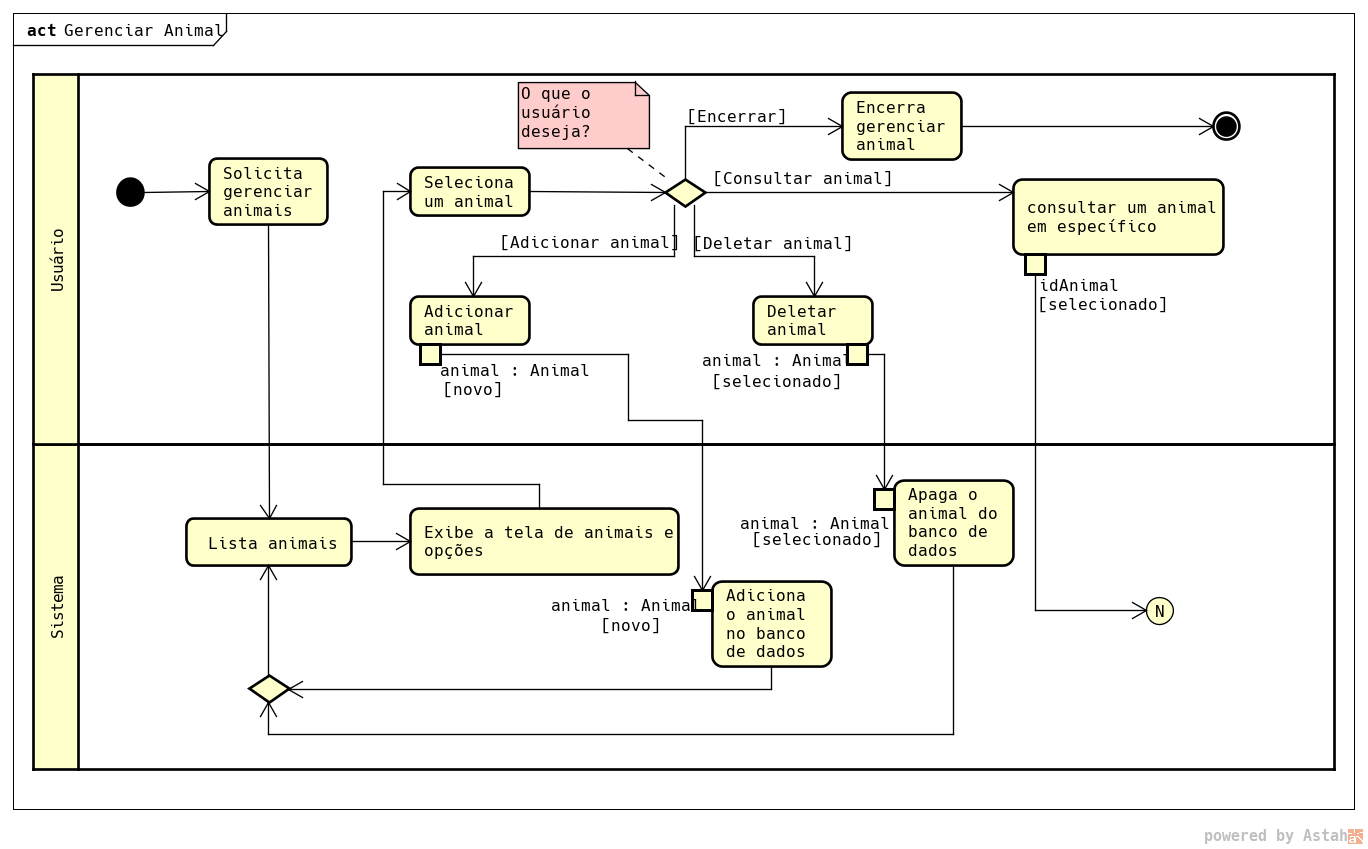
\includegraphics[width=\textwidth]{../img/GerenciarAnimal1.png}

		Fonte: Autoria própria.
	\end{center}
\end{figure}

\begin{figure}[H]
	\begin{center}
		\caption{Diagrama da Atividade de Gerenciar Animal parte 2}
		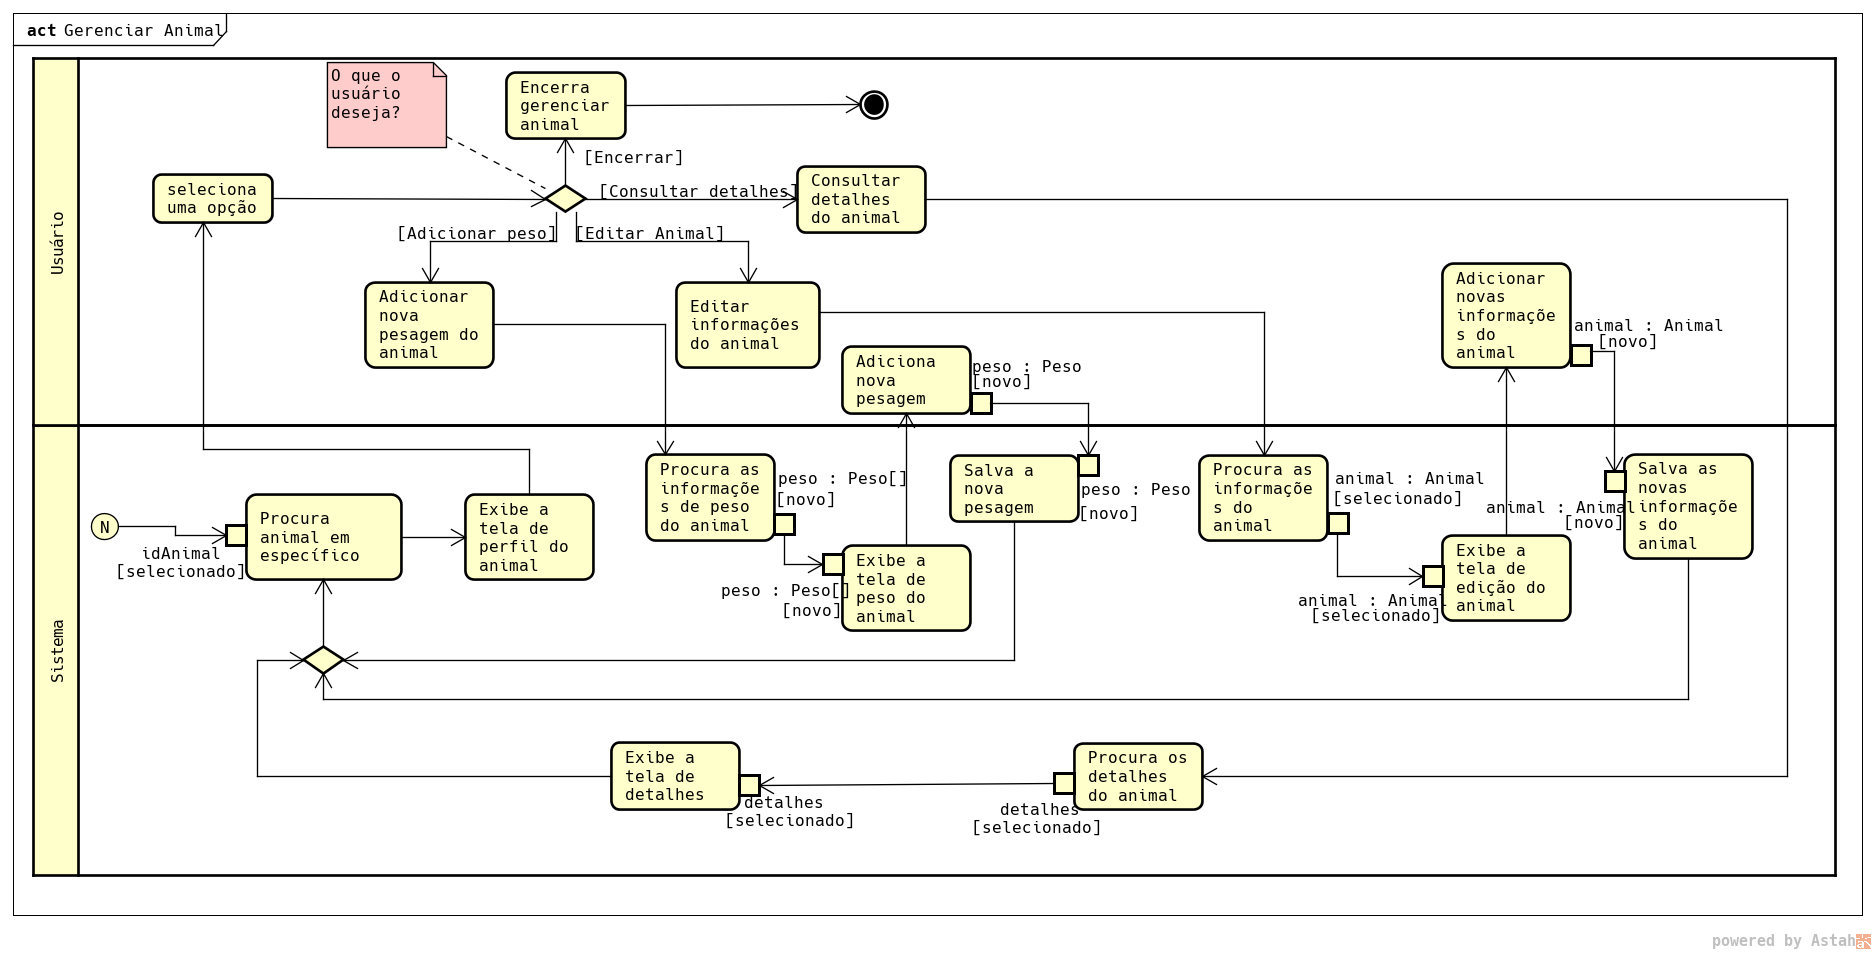
\includegraphics[width=\textwidth]{../img/GerenciarAnimal2.png}

		Fonte: Autoria própria.
	\end{center}
\end{figure}

\begin{figure}[H]
	\begin{center}
		\caption{Diagrama da Atividade de Gerenciar Remédios}
		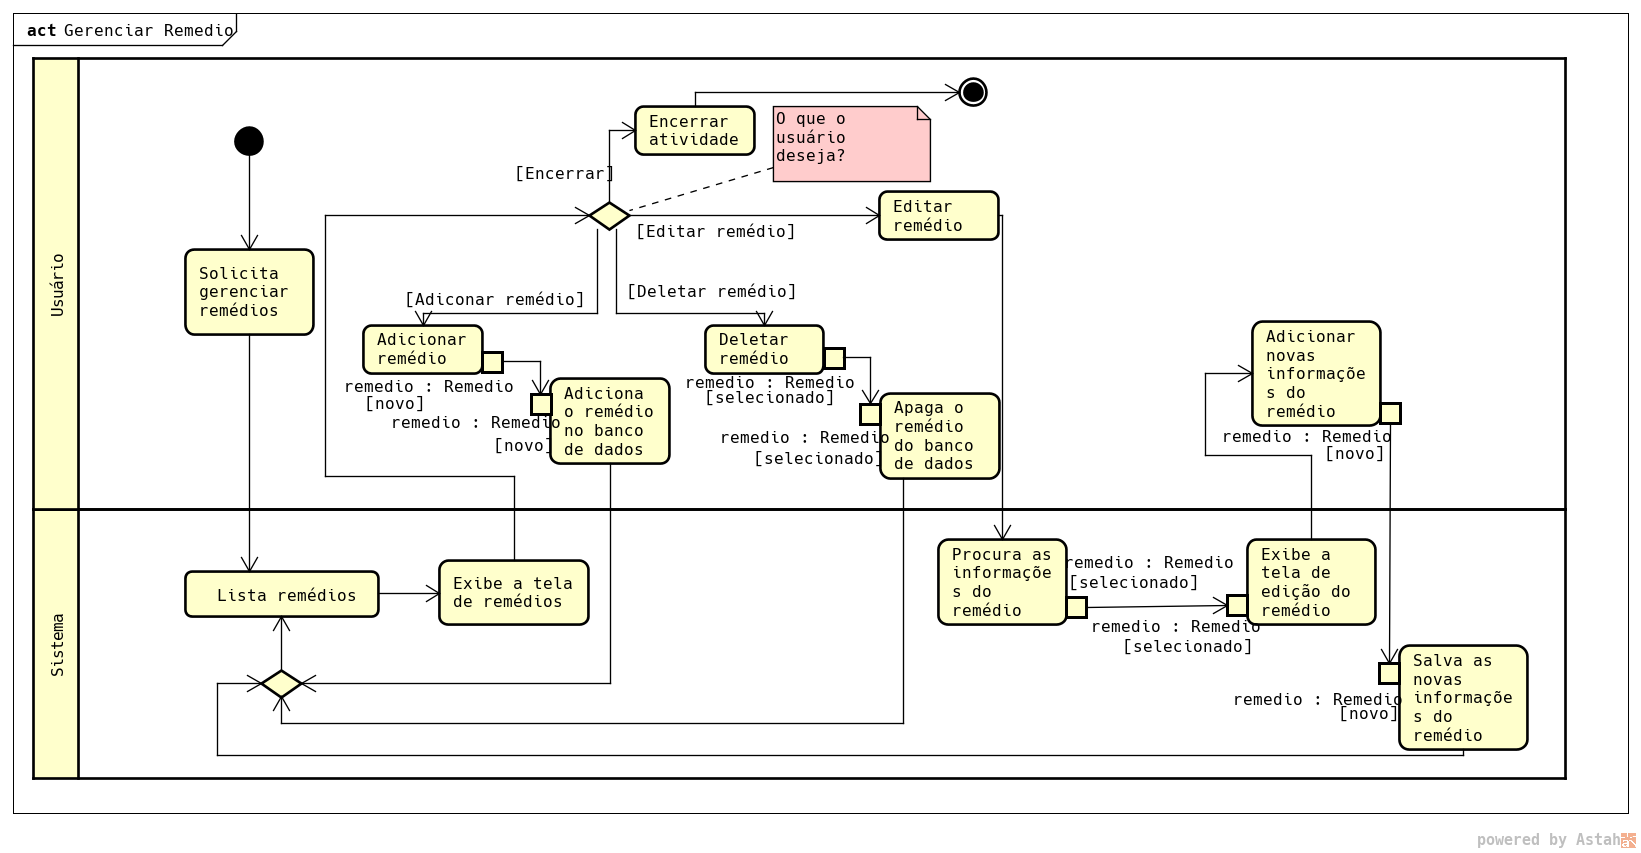
\includegraphics[width=\textwidth]{../img/GerenciarRemedio.png}

		Fonte: Autoria própria.
	\end{center}
\end{figure}

\begin{figure}[H]
	\begin{center}
		\caption{ Diagrama da Atividade de Gerenciar Medicações}
		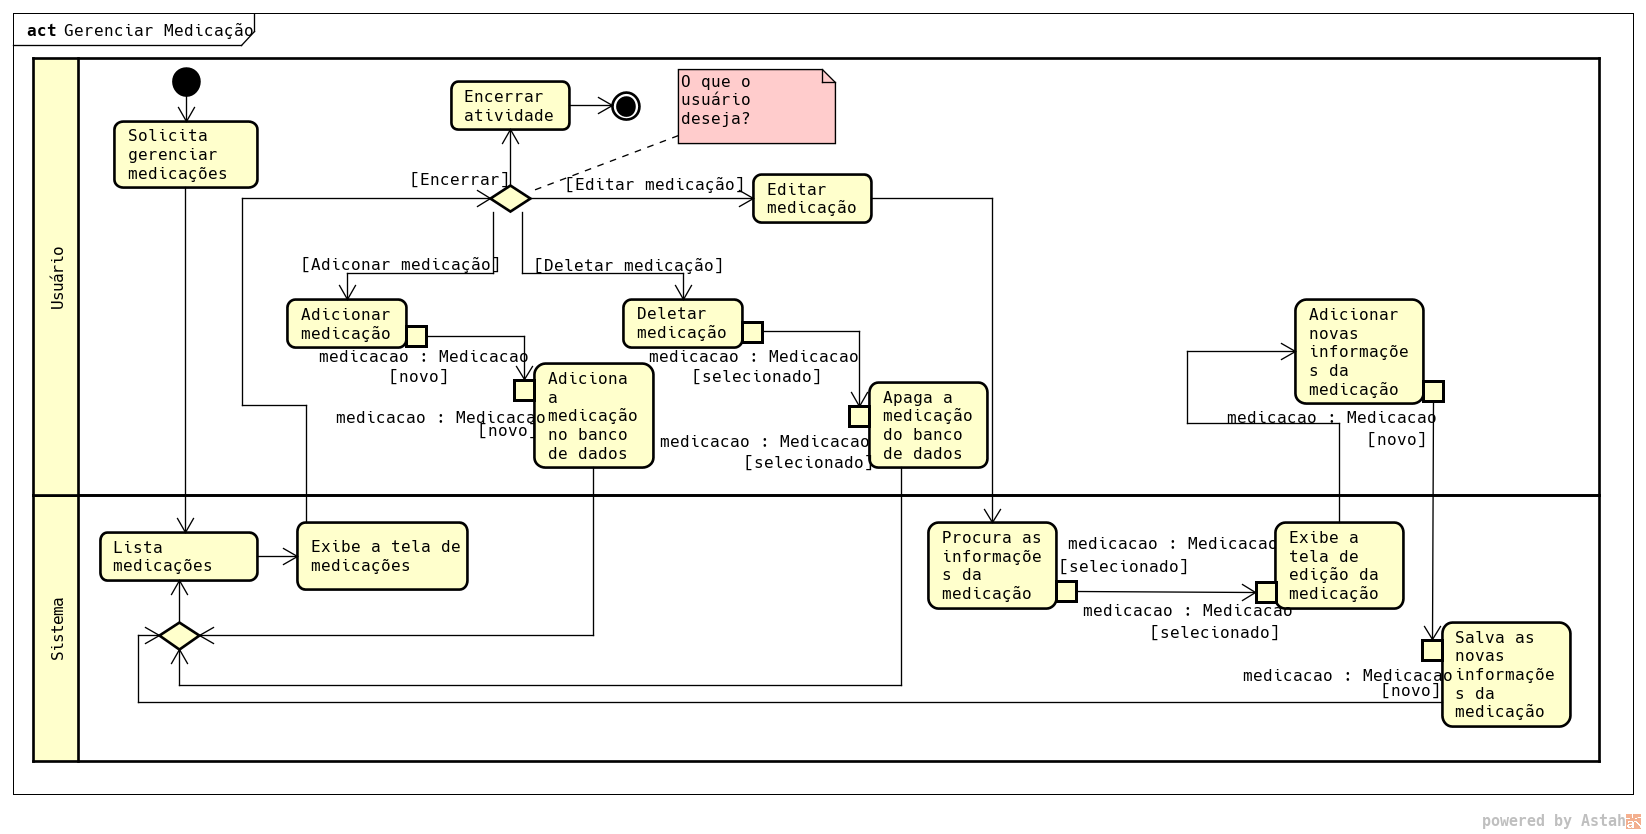
\includegraphics[width=\textwidth]{../img/GerenciarMedicacao.png}

		Fonte: Autoria própria.
	\end{center}
\end{figure}

\begin{figure}[H]
	\begin{center}
		\caption{Diagrama da Atividade de Visualizar Relatórios}
		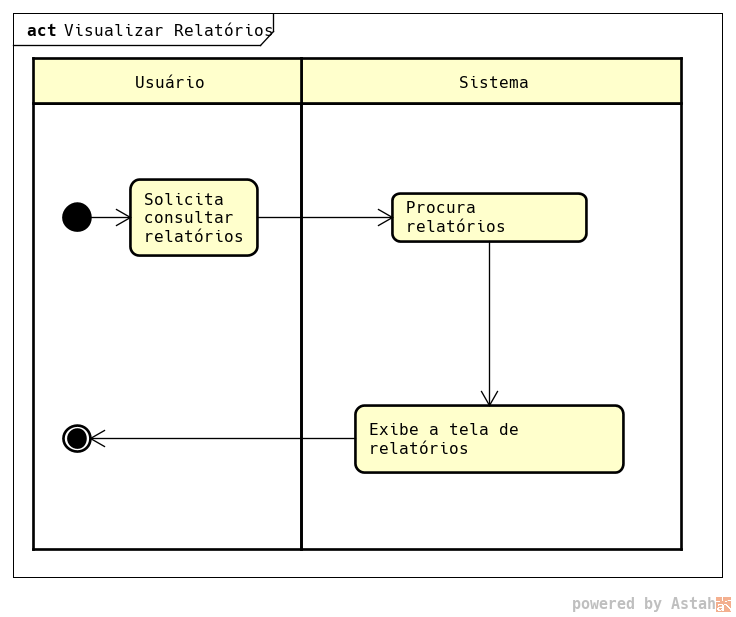
\includegraphics[width=\textwidth]{../img/Relatorios.png}

		Fonte: Autoria própria.
	\end{center}
\end{figure}

\chapter{ENTREVISTA COM UM DOS USUÁRIOS}\label{chap:entre}

\begin{itemize}
	\item \textbf{Você acha que o registro das informações da vida do animal bovino é útil?}
	\newline
	Sim. Pois garante que essas informações não se percam.

	\item \textbf{Quanto à visualização, você acredita que o histórico ajuda a gerenciar melhor os registros dos animais?}
	\newline
	Sim. Olhando o histórico é possível ter acesso rápido a quais foram os animais já foram medicados e quais ainda precisam da vacina.

	\item \textbf{O gráfico de peso auxilia na visualização das pesagens?}
	\newline
	Com certeza. É bem mais interessante olhar o crescimento ilustrado através do tempo. Ajuda a saber se estamos cuidando bem do animal, já que isso resulta uma subida grande no gráfico.

	\item \textbf{A possibilidade de exportar as informações de de sua fazenda para excel é uma funcionalidade útil?}
	\newline
	Sim, principalmente pela capacidade de manter um registro local, sem acesso a internet.

	\item \textbf{Você acredita que, em geral , o sistema é capaz de auxiliar no gerenciamento de animais de sua propriedade?}
	\newline
	Sim, o gerenciamento dos animais facilita o trabalho e possibilita o aumento da lucratividade da propriedade.

\end{itemize}


\end{apendicesenv}
